\documentclass{beamer}
\usepackage{tikz}
\usetikzlibrary{arrows,shadows,petri,decorations.markings,shapes}
\RequirePackage[many]{tcolorbox}
\usepackage{mathtools}
\begin{document}
 Das ist der Text vor
	\begin{tikzpicture}
    
	\node at (2,2){
\includegraphics[height=3cm]{images/logos/AquaDiva}};
	\node at (8,2){
\includegraphics[height=3cm]{images/logos/Minerva_green_text_en.pdf}};
	\node at (2,8){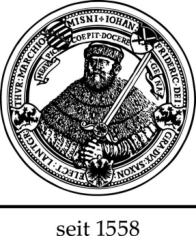
\includegraphics[height=3cm]{images/logos/Hanfried.pdf}};
	\node at (8,8){
\includegraphics[height=3cm]{images/logos/IMPRS_Logo__skalierbar.pdf}};
	\end{tikzpicture}
und nach dem Bildchen
\end{document}
